\documentclass[a4paper,11pt]{article}
\usepackage{fullpage}
\usepackage[latin1]{inputenc}
\usepackage[T1]{fontenc}
\usepackage[normalem]{ulem}
\usepackage[english]{babel}
\usepackage{listings,babel}
\usepackage{palatino}
\lstset{breaklines=true,basicstyle=\ttfamily}
\usepackage{graphicx}
\usepackage{moreverb}
\usepackage{url}
\usepackage{tweaklist}
\renewcommand{\itemhook}{\setlength{\topsep}{0pt}\setlength{\itemsep}{0pt}}

\title{Time to Digital Converter core for Spartan-6 FPGAs}
\author{S\'ebastien Bourdeauducq}
\date{August 2011}
\begin{document}
\setlength{\parindent}{0pt}
\setlength{\parskip}{5pt}
\maketitle{}
\section{Specifications}
The Time to Digital Converter (TDC) core is a high precision (sub-nanosecond) time to digital conversion core for Xilinx Spartan-6 FPGAs.

\begin{itemize}
\item Expected precision: 50-100ps (peak to peak).
\item Fixed point output:
\begin{itemize}
\item Integer part is number of FPGA clocks (coarse counter).
\item 13-bit fractional part (configurable with a VHDL generic).
\item With a 125MHz FPGA clock, LSB corresponds to 0.98ps.
\end{itemize}
\item Typical range: 268ms (using a <25.13>-bit value at 125MHz).
\begin{itemize}
\item Number of coarse counter bits configurable with a VHDL generic.
\end{itemize}
\item Latency: 6 cycles at 125MHz (not including host interface module).
\item Multiple channels.
\begin{itemize}
\item Configurable with a VHDL generic.
\item Calibration logic shared between channels.
\end{itemize}
\item Reports both rising and falling edges of the input signal.
\item Input signal must not have transitions shorter than the FPGA clock period (e.g.\ the frequency of the input signal must be less than half of the FPGA clock).
\item Uses a counter for coarse timing and a calibrated delay line for fine timing.
\item Delay line implemented with carry chain (\verb!CARRY4!) primitives.
\item Calibration mechanism:
\begin{itemize}
\item at startup (and after receiving a reset command), send random pulses into the delay line (coming from e.g. a on-chip ring oscillator), build histogram, compute delays (as explained in the Fermilab paper \cite{fermilab}, initialize the LUT, and measure the frequency of the compensation ring oscillator.
\item for online temperature/voltage compensation, measure again the frequency of the ring oscillator, compare it to the frequency measured at start-up, linearly interpolate the delays, and update the LUT.
\end{itemize}
\item "Wave union" not implemented.
\item Input signals (without host interface module):
\begin{itemize}
\item Input signal.
\item Calibration signal.
\item Coarse counter reset.
\item Per-channel de-skew value.
\item Full reset (and recalibrate).
\item Clock.
\end{itemize}
\item Output signals (without host interface module):
\begin{itemize}
\item Startup calibration in progress.
\item Periodic counter overflow.
\item Received rising/falling edge notification:
\begin{itemize}
\item Strobe signal.
\item Rising/falling edge.
\item Fixed point timestamp.
\item Raw encoded value from the delay line.
\end{itemize}
\end{itemize}
\item Debug interface:
\begin{itemize}
\item Forced switch to the calibration signal.
\item Access to the histogram values from the startup calibration.
\item Access to the frequencies of the online calibration ring oscillators.
\end{itemize}
\item Optional host/CPU interface module:
\begin{itemize}
\item Wishbone slave.
\item Configuration and status registers.
\item Interrupts: edge received, counter overflow.
\end{itemize}
\end{itemize}

\section{Architecture}
\subsection{Overview}
The block diagram of the core is given in Figure~\ref{fig:block}.

\begin{figure}[h]
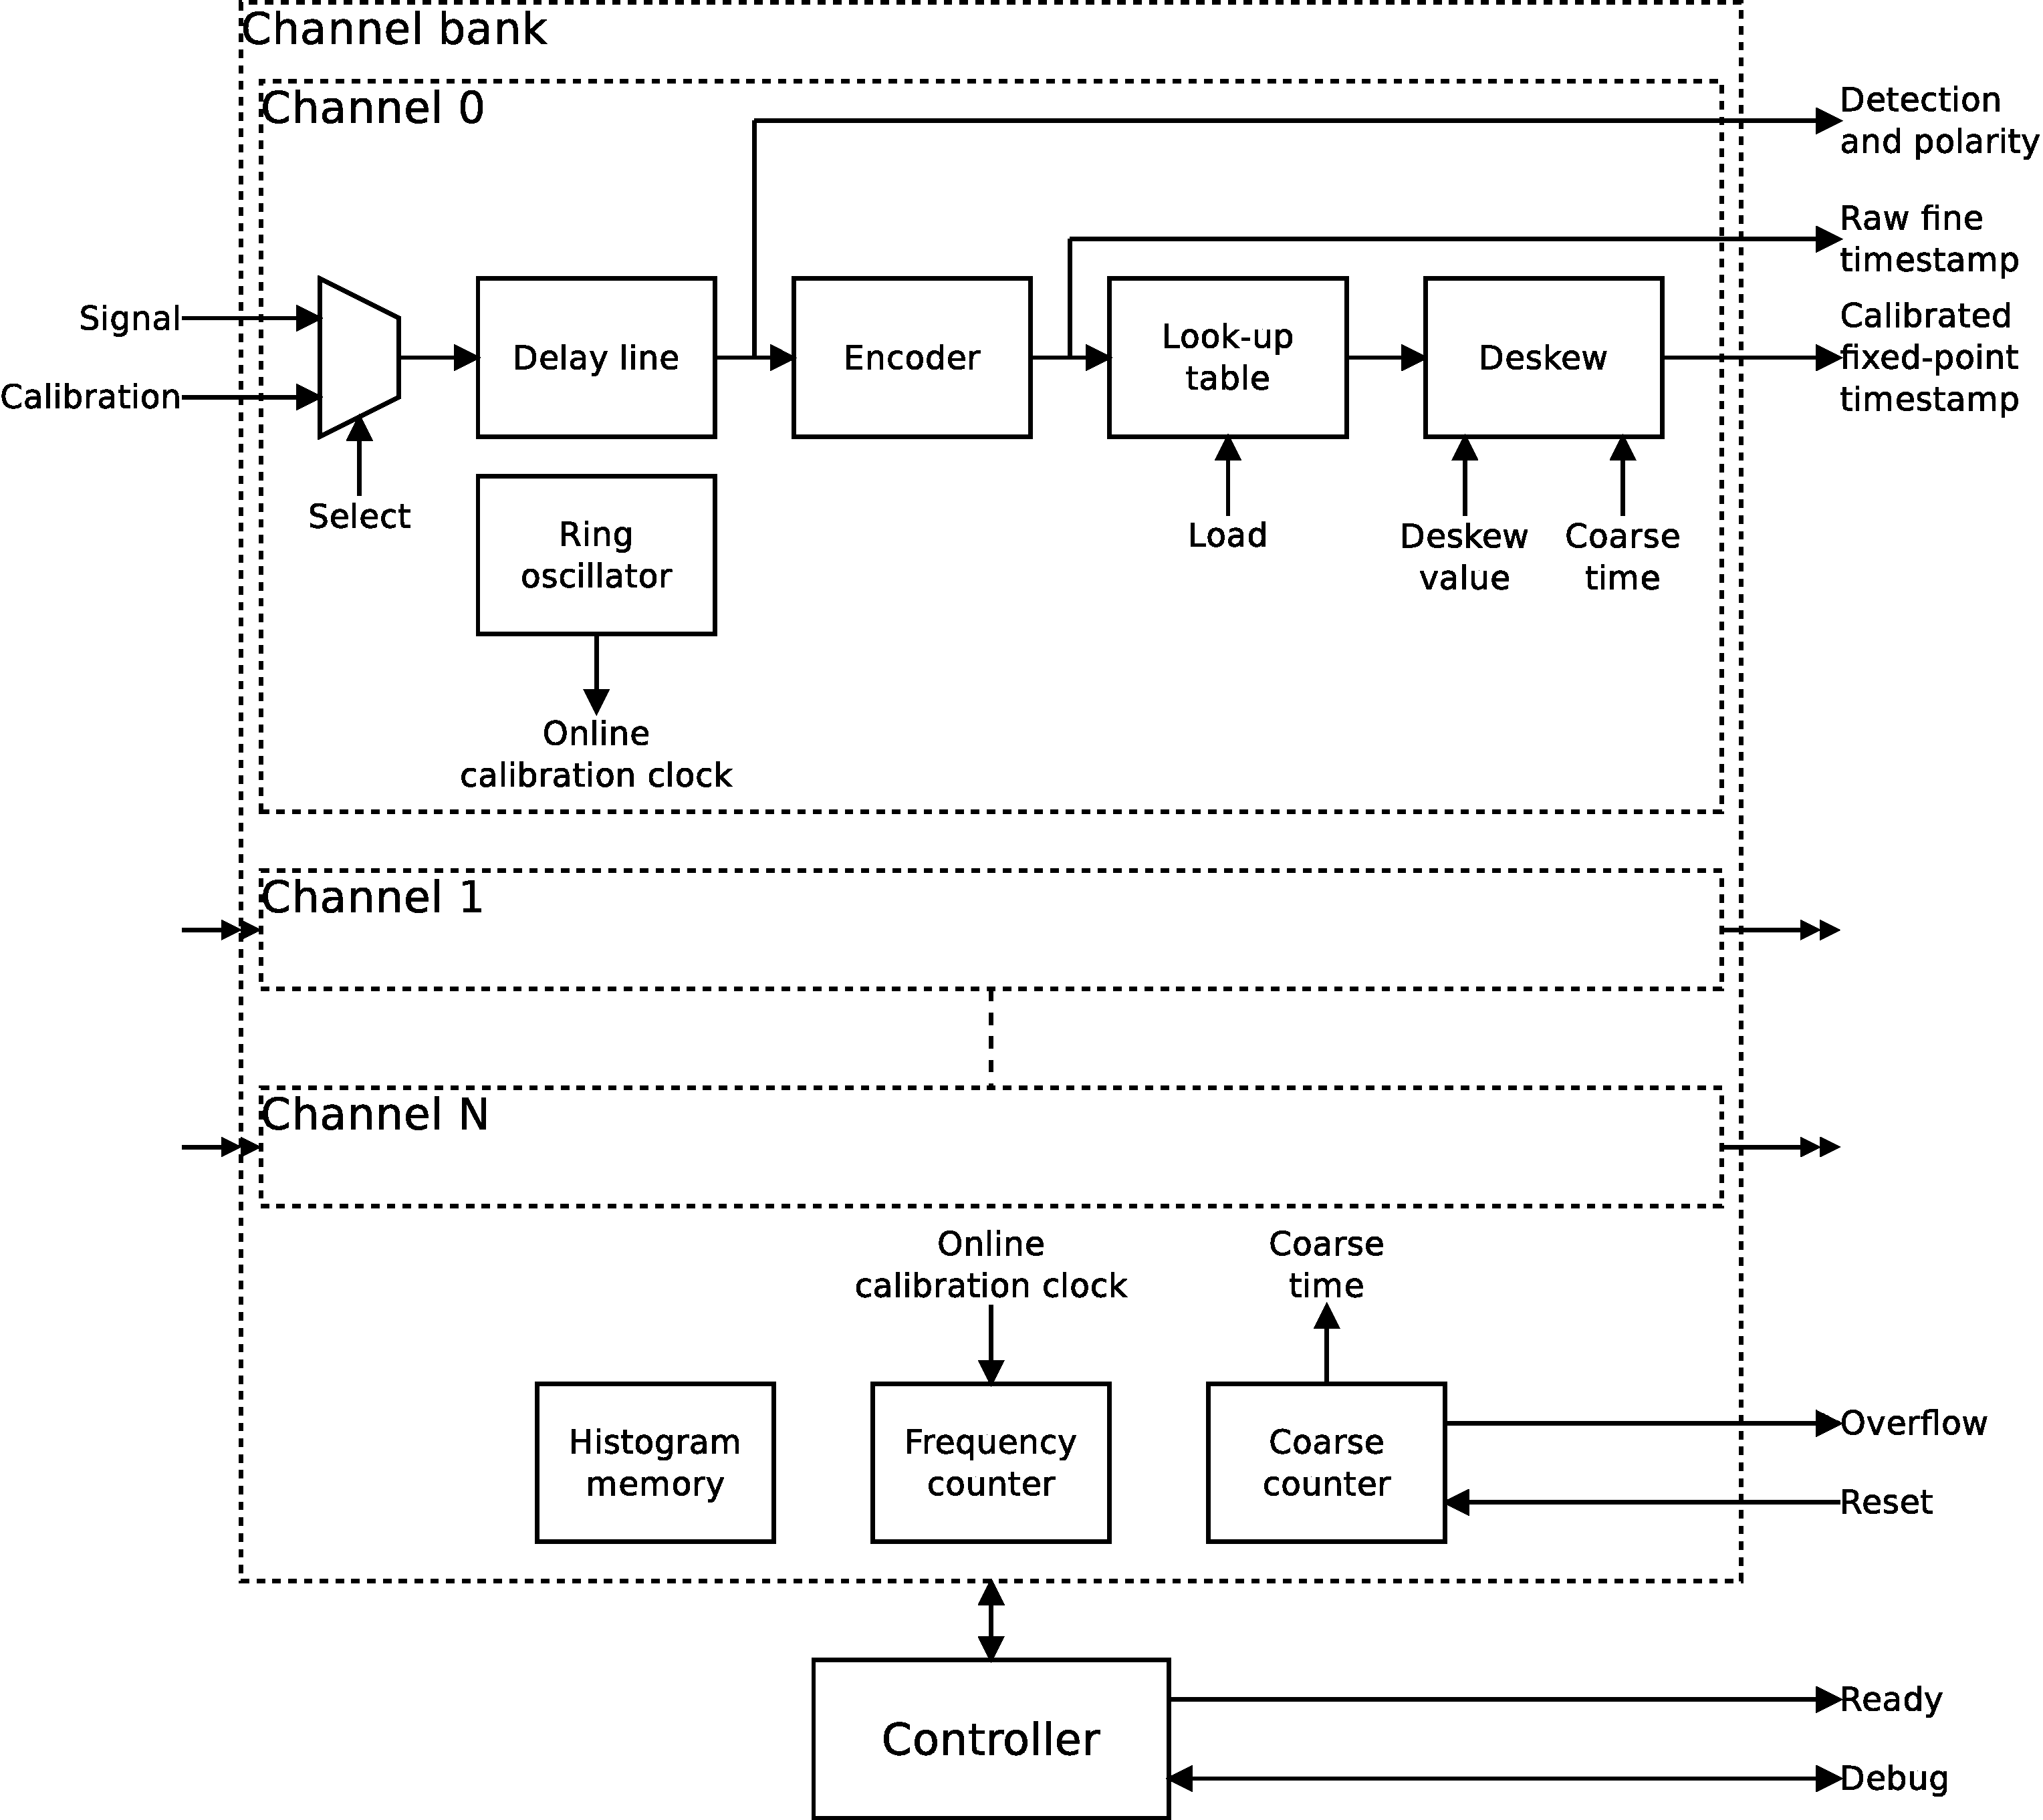
\includegraphics[width=\textwidth]{block.pdf}
\caption{Block diagram of the TDC core.}
\label{fig:block}
\end{figure}

The signal to be timestamped is injected into a tapped delay line to obtain a fine time measurement (below the clock period). The total delay of the delay line must be greater than the clock period. At each clock tick, an encoder counts the taps the signal has reached and gives a \textit{raw} measurement of the timestamp of the signal within the current clock cycle. This raw value is fed into a look-up table (LUT) which converts it into a calibrated value expressed in subdivisions of the clock cycle, called the \textit{fractional} value. Finally, in the \textit{deskew} stage, the fractional value is combined with the index of the current clock cycle given by the coarse counter, and the resulting fixed-point value is added a user-defined constant to enable the TDC core to directly generate timestamps relative to the source of the system clock.

The main difficulty with this system is that the delay line is subject to process, temperature and voltage (PVT) induced variations, and it needs to be calibrated against them.

To generate the LUT contents, the controller switches to the calibration signal. The key property of the calibration signal is that the probability density of its transition timestamps within a system clock cycle must be constant. The controller measures the raw timestamps and books a histogram. Because of the constant probability density, the heights of the histogram bars are approximately proportional to the delays between the taps of the delay line after enough measurements have been taken. Further, the last tap to have recorded a signal transition corresponds to a delay equal to the system clock period. This enables the controller to build the initial contents of the LUT. This process is called \textit{startup calibration}.

The drawback of the startup calibration is that the system cannot operate while the calibration is taking place. Therefore, a process of \textit{online calibration} has been devised. Each channel contains a ring oscillator that is placed close to the delay line. The controller periodically measures the frequency of this ring oscillator, compares it to the frequency that was measured at the time of startup calibration, linearly interpolates the fractional timestamps, and updates the LUT. This allows compensation of temperature and voltage effects while the system keeps running.

The system gives timestamps of both rising and falling edges of the incoming signal. The rising edges are discerned from the falling edges using the ``polarity'' output.

\subsection{Delay line structure}
The delay line uses a carry chain. It is made up of \verb!CARRY4! primitives whose \verb!CO! outputs are registered by the dedicated D flip flops of the same slices. The signal is injected at the \verb!CYINIT! pin at the bottom of the carry chain. The \verb!CARRY4! primitives have their \verb!S! inputs hardwired to 1, which means the carry chain becomes a delay line with the signal going unchanged through the \verb!MUXCY! elements (see \cite{s6hdl} for reference). Since each \verb!CARRY4! contains four \verb!MUXCY! elements, the delay line has four times as many taps as there are \verb!CARRY4! primitives.

Using the Xilinx timing model, a surprising observation is that some delay differences between consecutive taps are negative. This probably is at the origin of the ``bubbles'' mentioned in the EPFL paper \cite{epfl}. The schematics given by Xilinx of the \verb!CARRY4! primitive is misleading there, and has probably little to do with the actual transistor-level implementation. The Xilinx documentation \cite{s6hdl} gives a hint by describing the primitive as ``Fast Carry Logic \textit{with Look Ahead}''.

To avoid negative differences, we simply reorder the bits at the output of the delay line to sort the taps by increasing actual delays. We can then think of the delay line according to Figure~\ref{fig:delaystruct}. The bin widths are uneven, but the incoming signal reaches the taps in order. This last property simplifies the encoder design, since it only has to count the number of identical bits at the beginning of the delay line.

\begin{figure}[h]
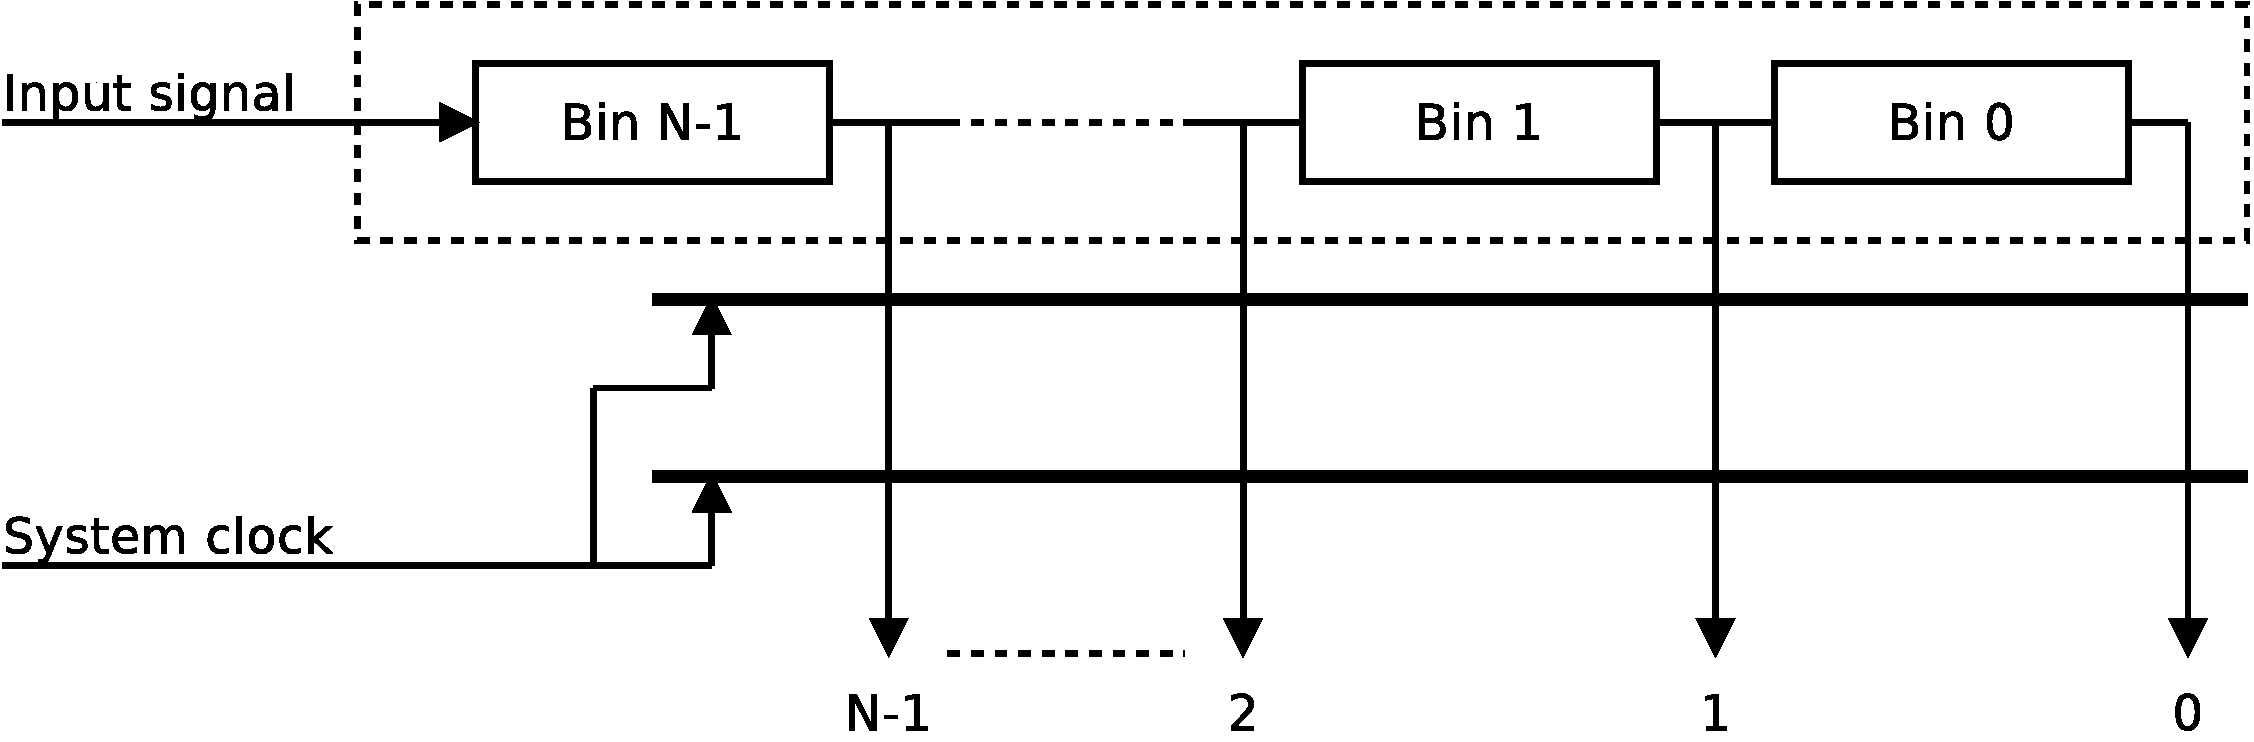
\includegraphics[width=\textwidth]{delaystruct.pdf}
\caption{Representation of the delay line.}
\label{fig:delaystruct}
\end{figure}

\subsection{Calibration details}
In the formulas below:
\begin{itemize}
\item $T_{sys}$ is the system clock period.
\item $H(n)$ is the number of hits in the histogram at output $n$. A hit at output $n$ means that the signal propagated down to output $n$, without reaching output $n-1$.
\item $W(n)$ is the width of bin $n$.
\item $C = \displaystyle\sum\limits_{n=0}^{N-1} H(n)$ is the total number of hits in the histogram.
\item $R(n)$ is the timestamp of an event whose signal propagated down to output $n$ (without reaching output $n-1$), measured backwards from the clock tick.
\item $f$ (respectively $f_{0}$) is the current (respectively reference) frequency of the online calibration ring oscillator.
\end{itemize}

\subsubsection{Offline calibration}
We take the first output of the delay line to be the origin of the time measurements, and we define:
\begin{equation}
W_{0}(N-1) = 0
\end{equation}

The width of other bins is proportional to their respective number of counts in the histogram. The widths sum up to a clock period. This leads to the following equation:
\begin{equation}
W_{0}(n) = \frac{H(n+1)}{C} \cdot T_{sys}
\end{equation}

The timestamp is the sum of the widths of the traversed bins:
\begin{equation}
R_{0}(n) = \displaystyle\sum\limits_{i=n}^{N-1}{W_{0}(i)} = \frac{T_{sys}}{C} \cdot \displaystyle\sum\limits_{i=n}^{N-1}{H(i)}
\end{equation}

In the TDC core, the unit is the clock period, and the output has $F$ base 2 digits after the radix points. The controller also chooses\footnote{This choice was made for design simplicity reasons, and the precision can be improved by increasing C.} $C=2^F$. Expressed in units of $2^{-F}$ clock periods (which is the weight of the least significant bit of the fixed-point output), we have:
\begin{equation}
\frac{T_{sys}}{C}=1
\end{equation}

\subsubsection{Online calibration}
Online calibration is performed with a simple linear interpolation of the delays relative to the ring oscillator frequencies:
\begin{equation}
R(n) = \frac{f_{0}}{f} \cdot R_{0}(n)
\end{equation}

Note that when $f < f_{0}$, some values can go above the maximum fractional part value of $1 - 2^{-F}$ and might not fit in the LUT anymore. To solve this problem, all LUT values contain a configurable amount of \textit{guard bits}, which are integer part bits used to contain the overflow when the situation appears.

\section{Implementing the core}
\subsection{Generics}

\subsection{Ports}

\subsection{Synthesis and physical implementation}
\subsubsection{False timing paths}
The calibration selection signal is driven synchronously by the controller, and the output of the multiplexer goes through the delay line before being recaptured synchronously by the input flip-flops. The automatic place and route tool incorrectly assumes this is a regular synchronous path. Since the delay line is always longer than a clock period, it aborts with a message saying that the components delays alone exceed the timing constraints. The problem is resolved by adding ``timing ignore'' (TIG) constraints into the UCF file, using a syntax based on the example below:
\begin{verbatim}
NET "cmp_channelbank/g_channels[0].cmp_channel/muxed_signal" TIG;
\end{verbatim}

One such constraint must be added per channel, and the number ``0'' incremented accordingly.

\subsubsection{Delay line placement}
The delay line must be placed in a way that minimizes the delay from the input signals IOBs. The reason is that this delay is affected by PVT variations that are not compensated for.

\subsubsection{Ring oscillator placement}
To be most effective, the ring oscillator must be placed close to the delay line of the same channel.

\section{Host interface module}

\begin{thebibliography}{99}
\bibitem{s6hdl} Xilinx, \textsl{Spartan-6 Libraries Guide for HDL Designs}, \url{http://www.xilinx.com/support/documentation/sw_manuals/xilinx12_3/spartan6_hdl.pdf}
\bibitem{epfl} Claudio Favi and Edoardo Charbon, \textsl{A 17ps Time-to-Digital Converter Implemented in 65nm FPGA Technology}, ACM 2009, \url{http://infoscience.epfl.ch/record/139431}
\bibitem{fermilab} Jinyuan Wu and Zonghan Shi, \textsl{The 10-ps Wave Union TDC: Improving FPGA TDC Resolution beyond Its Cell Delay}, IEEE 2008, \url{http://www-ppd.fnal.gov/EEDOffice-W/Projects/ckm/comadc/PID765918.pdf}
\end{thebibliography}

\end{document}
